% =====================================================================
%  P1 — Single-channel consumer EEG: what it can and cannot measure
%  Status: draft v4.0 (2026-11-06). Every number comes from results/*.json.
%  Analysis plan is planned but NOT registered (see PREREGISTRATION.md).
%  Build: latexmk -pdf -interaction=nonstopmode -halt-on-error main.tex
% =====================================================================
\documentclass[11pt,a4paper,twocolumn]{article}

\usepackage[T1]{fontenc}
\usepackage[utf8]{inputenc}
\usepackage[english]{babel}
\usepackage[margin=2.5cm]{geometry}
\usepackage{amsmath,amssymb}
\usepackage{textcomp}
\usepackage{graphicx}
\usepackage[colorlinks=true,linkcolor=blue,citecolor=blue,urlcolor=blue]{hyperref}
\usepackage{caption}
\usepackage{multicol}
\usepackage{float}

\title{What Single-Channel and Low-Cost EEG\\
Can and Cannot Measure:\\[2pt]
A Reproducible Degradation Benchmark\\
and Reporting Protocol}
\author{Eyy\"ub G\"uven\thanks{\texttt{eyyub.gvn@gmail.com}. ORCID 0009-0005-6017-8622.}}
\date{\today}

\begin{document}

\makeatletter
\twocolumn[{
\begin{@twocolumnfalse}
\maketitle
\begin{abstract}
\noindent
Cheap EEG headsets now appear in classrooms, clinics and living rooms, often with claims
about attention, relaxation and emotion. The hardware is capable; the reporting around
it is not. A recording made with one dry electrode, a low sampling rate and an unknown
noise floor cannot be interpreted without knowing how each of those choices changes the
analysis. We built a benchmark that starts from open high-density recordings and walks
them down, step by step, to a single-channel consumer setting: one electrode, 128\,Hz,
1\,\textmu V quantisation, 1--40\,Hz bandwidth, pink noise at 20/10/5/0\,dB and
synthetic blinks at 5/15/30 per minute. We then asked which standard analyses survive.
In all 109 subjects of the EEG Motor Movement/Imagery Dataset, alpha reactivity was
almost unchanged by the acquisition chain when the reference came from the same
electrode (99.99\% retained; 95\% CI $[0.9996, 1.0001]$), while choosing a frontal site
cost about 42\% of eyes-closed alpha power (Fz/posterior ratio $0.58$). Noise mattered:
at 0\,dB the effect fell to 59\% of the reference. Our additive blink model changed the
estimate by about 0.2\%, but it cannot test real ocular artifacts. In 18 high-end
recordings from an open affective dataset, valence, arousal and four-quadrant decoding
were above chance with the full montage ($0.69$, $0.68$, $0.58$). With one electrode,
valence was no longer detectable ($0.52$; equivalence untested), arousal weakened
($0.56$; $q=0.050$ in the six-contrast family) and four-class accuracy fell to $0.34$
(above the $0.25$ chance level but far below the montage). None of four midline sites
rescued valence, and a band control showed that part of the montage advantage depends
on beta-band features, possibly muscle activity. A 14-channel consumer headset
performed similarly to the matched high-end montage ($0.67$/$0.71$ versus $0.73$/$0.66$
on the 12 shared participants), although a $\pm10$-point equivalence test did not pass.
Short-lag alpha stability was low ($r_{SB}=0.016$); block-level alpha power was stable
(ICC(2,1)$=0.92$). The motor arm was invalid because its reference decoder did not
exceed chance. We provide the code, derived results, decision matrix and reporting
checklist.
\end{abstract}

\noindent\textbf{Keywords:} consumer EEG, single-channel, reproducibility, benchmark,
affective decoding, reporting standards
\end{@twocolumnfalse}
}]
\makeatother

\section{Introduction}
% 01-introduction — v4.0
\subsection*{A device in search of a method}
Low-cost EEG headsets are sold as attention trainers, relaxation aids, sleep gadgets and
emotion sensors. Some of them record real neural signal: consumer devices have been
validated against research amplifiers for event-related potentials
\citep{krigolson2017muse,badcock2015emotiv}, and resting-state comparisons show that
spectral estimates and test--retest behaviour differ across systems
\citep{ratti2017comparison,cannard2021muse}. The problem is what happens after the
recording. A paper may report that alpha power increased during relaxation without
saying which electrode was used, how the signal was filtered, whether blinks were
removed, or how the result compares with a conventional montage. A reader cannot tell
whether the finding reflects a cognitive process or an artefact of the recording setup.

This matters for two reasons. First, the same claim can be produced by very different
pipelines, so the result is difficult to reproduce. Second, a single frontal electrode
picks up cortical activity together with eye movements and muscle noise
\citep{whitham2007emg}; presenting that mixture as a specific cognitive measure invites
overclaiming. Device-comparison studies are useful, but they answer a different
question: whether one headset is close enough to a reference amplifier under one
protocol. They do not tell a reader which analyses still work when the acquisition is
reduced.

\subsection*{What this paper does}
We take high-quality open recordings and degrade them one step at a time towards what a
cheap headset provides. The steps are explicit: a single electrode, 128\,Hz sampling,
1\,\textmu V quantisation, 1--40\,Hz band-limiting, pink noise at four levels, and
synthetic blinks at three rates. Each step is reported separately, so a reader can see
which manipulation matters. The benchmark has four analysis families: alpha
reactivity, affective decoding, motor decoding (exploratory) and reliability. The
reference is always the same recording before degradation, and, where it matters, the
same electrode rather than a whole-head average.

Two open datasets make this feasible. The EEG Motor Movement/Imagery Dataset provides
109 subjects, 64 channels and eyes-open and eyes-closed baselines
\citep{schalk2009eegbci}. An open affective dataset contains 20 participants recorded
simultaneously with a low-cost Emotiv EPOC+ and a high-end BrainVision system, with
valence--arousal quadrant labels \citep{sanchezreolid2022emotion,sanchezreolid2025dataset}.
The first dataset is used for the degradation grid; the second lets us compare a real
low-cost device with a high-end montage and with the same high-end data reduced to one
electrode.

\subsection*{What we find}
The results are mixed, and the mix is the point. Alpha reactivity is robust to the
acquisition chain: once the reference is taken at the same electrode, 99.99\% of the
effect remains. The choice of electrode, however, costs about 42\% of eyes-closed alpha
power, and noise reduces the effect monotonically. In the affective data, the full
montage decodes valence, arousal and quadrant above chance, but a single electrode does
not: valence is no longer detectable, arousal weakens, and four-class accuracy drops
close to the level expected from a weak classifier. A band control suggests that part of
the montage advantage comes from beta-band features, which may include muscle activity.
A 14-channel Emotiv performs about as well as the high-end montage in this sample, but
the equivalence test does not pass, so the comparison remains descriptive.

The contributions are: a reproducible degradation pipeline; a decision matrix that maps
each result to a claim-level verdict; a same-site retention estimate for alpha; a
decomposition of the affective result into representation, site and band effects; and a
reporting checklist for single-channel studies, based on COBIDAS MEEG
\citep{pernet2020cobidas}, EEG-BIDS \citep{pernet2019bids} and the CRED-nf checklist
\citep{ros2020crednf}. The code, the derived results and the JSON files behind every
number are archived with the paper.

The paper is not a clinical or wellness intervention study, and it does not validate a
commercial product. It is a methods study: it measures what different analyses can
support, and it shows where the limits lie.


\section{Related Work}
% 02-related
\subsection*{Consumer and low-cost EEG validation}
Comparisons of medical-grade and consumer wireless systems report that consumer
hardware can recover common event-related components under favourable conditions,
while signal quality and artifact susceptibility differ substantially between devices
and sessions \cite{ratti2017comparison,krigolson2017muse,sawangjai2020consumer}. One of
the closest prior studies compared four systems (including MindWave and Muse) on five
participants across two visits, focusing on Fp1 and explicitly comparing eyes-closed
and eyes-open spectra and their test--retest reliability
\cite{ratti2017comparison}. That is close to our alpha arm on real hardware, so the gap
cannot be "nobody has looked at consumer spectral reliability"; the gap is that
existing work does not quantify which analyses survive a \emph{controlled} degradation
chain, and does not connect that chain to claim-level verdicts. Work on channel subsets for emotion decoding has shown that small, well-chosen
montages can be competitive with large ones \cite{zheng2015channels}; what is missing is
a controlled degradation of the same recordings with a site-matched reference and a
claim-level decision rule. Our contribution is therefore the decomposition and the
decision matrix, not the observation that fewer channels can hurt.

\subsection*{Reproducibility and reporting standards}
Psychology and neuroscience face a well-documented reproducibility problem
\cite{osc2015reproducibility}. In electrophysiology the community response has been
standardised reporting (COBIDAS MEEG) \cite{pernet2020cobidas} and standardised data
organisation (EEG-BIDS) \cite{pernet2019bids}. Both are written primarily for
research-grade acquisitions; they specify what to report, but not what can be
inferred when the acquisition is a single channel. The present benchmark is designed
to fill that inference gap and to make the reporting checklist operational for
consumer-device studies.

\subsection*{Analysis pipelines and artifact handling}
Modern open pipelines make preprocessing explicit and reproducible
\cite{gramfort2013mne,delorme2004eeglab,oostenveld2011fieldtrip}, and automated
artifact rejection and independent-component classification reduce researcher degrees
of freedom \cite{jas2017autoreject,piontonachini2019iclabel}. These tools assume
enough channels for spatial decomposition; with one channel, ICA is unavailable and
most artifact rejection reduces to amplitude thresholds or regression against
auxiliary signals. A benchmark of single-channel conditions therefore must treat
artifact handling as part of the independent variable, not as a preprocessing detail.

\subsection*{Feature validity and open data}
Band-power features are the workhorse of consumer-EEG claims, and their test--retest
reliability is a prerequisite for any individual-level interpretation. Open datasets
with repeated conditions and affective ratings allow reliability and decoding to be
measured against a known ground truth rather than asserted
\cite{schalk2009eegbci,koelstra2012deap}. We build directly on the EEGBCI resources and
on an open affective dataset that contains both low-cost and high-end recordings
\cite{sanchezreolid2022emotion,sanchezreolid2025dataset}; DEAP and DREAMER are discussed
as alternatives that could not be used. We report every degradation step so that a
reader can map our results onto their own acquisition.

\subsection*{Positioning}
Relative to device-comparison work, our contribution is analysis-centred and
degradation-based. Relative to reporting standards, it is quantitative: rather than
saying which variables to report, it estimates what each variable is worth under
single-channel constraints. To our knowledge, no existing benchmark reports, for the
same open datasets, how alpha reactivity, single-trial decoding, reliability and blink
susceptibility change as a function of explicit consumer-hardware degradations.

\subsection*{Benchmarking methodology}
The idea of comparing analysis pipelines on shared datasets is established in BCI
research: MOABB provides trustworthy benchmarking across datasets and pipelines
\cite{jayaram2018moabb}. Our benchmark differs in object --- it holds the pipeline
approximately fixed and varies the acquisition conditions, rather than comparing
algorithms --- but it inherits the principle that a claim about a method should be
evaluated against a common, open reference. Filter design is a concrete example of
why this matters: apparently small high-pass choices can create artifactual effects
and incorrect conclusions \cite{tanner2015filters}, which is exactly the kind of
degradation our chain isolates and reports.


\section{Methods}
% 03-methods — v1.0
\subsection*{Datasets}
\textbf{EEG Motor Movement/Imagery Dataset} \citep{schalk2009eegbci}. All 109 subjects were used: 64 channels at 160\,Hz, runs 1--2 for the
eyes-open and eyes-closed baselines and runs 4, 8 and 12 for imagined left/right hand
movement, as defined in the dataset documentation. Motor decoding uses the ten subjects for whom the imagery runs
were degraded in this pass, and is treated as exploratory.

\textbf{Affective dataset} \citep{sanchezreolid2022emotion,sanchezreolid2025dataset}.
The open CC BY 4.0 dataset from Zenodo 14787743 contains EEG from 20 participants who
viewed International Affective Picture System images selected to induce four
valence--arousal quadrants, recorded with a low-cost Emotiv EPOC+ and a high-end
BrainVision system. The archive's \texttt{EEG/Experiment\_files} directory contains 18 BrainVision
recordings (66 channels, 500\,Hz, sampling interval 2000\,\textmu s); a nineteenth
recording sits in a separate \texttt{EEG registro\_nuevo} folder and was not used. All
18 recordings in the analysed directory completed the pipeline. The files are named
\texttt{eegbci<subject>-<session>} by the archive; this is the archive's own naming for
the affective recordings and does not refer to the EEGBCI motor dataset. The
valence/arousal labels come from the affective picture protocol, not from a motor task. BrainVision
marker codes map to the quadrants as follows: 1 = high valence/high arousal,
2 = low valence/high arousal, 3 = high valence/low arousal, 4 = low valence/low
arousal, 10/14 = neutral. Each recording contains approximately 10 trials per quadrant
and 8 neutral trials; neutral trials are excluded from valence and arousal analyses.
Quadrant labels are the normative assignments of the International Affective Picture
System \citep{lang2008iaps}, not participants' own ratings.
Marker positions are used as onsets and each trial is epoched 0--2.5\,s after onset.
The low-cost Emotiv arm is analysed for the 12 participants whose CSV files are
usable in the distributed archive (five files are empty or header-only and three fail
the timestamp alignment). The device has been used in validation work on
event-related potentials \citep{badcock2015emotiv}. The files contain 14 EEG channels at
128\,Hz in device units with absolute wall-clock timestamps. The log session whose
absolute trial times fall inside the CSV span is selected; trials are aligned by
converting each log onset to an absolute time (SessionStartDateTimeUtc plus the
millisecond onset) and matching it to the nearest CSV sample, with a clock offset chosen
from $\{0,\pm1,\pm2\}$ hours by maximising the number of trials inside the recording
span. Emotiv epochs run from $-0.2$ to $+2.3$\,s around the aligned sample (the
BrainVision epochs run 0--2.5\,s), and the same band-power and LDA pipeline is applied.
The median absolute difference between a log onset and its nearest CSV sample was
25\,ms (95th percentile 59\,ms, maximum 70\,ms; stored per subject in
\texttt{results/emotiv.json}), and no trial exceeded the 1\,s alignment screen (this is a timestamp screen, not an amplitude rejection threshold). The
two condition arms in the archive are not otherwise distinguished. This yields a
three-way comparison: high-end full montage, low-cost 14-channel headset, and high-end
data reduced to a single degraded channel.

Both datasets are de-identified and openly available. No new data were collected.

\subsection*{Degradation grid}
EEGBCI recordings are processed at a full-montage reference and at twelve
single-channel conditions: a cumulative acquisition chain (Fz; +128\,Hz; +1\,\textmu V
quantisation; +1--40\,Hz band-limiting), a noise arm (20/10/5/0\,dB pink noise, no
blinks; pink noise is a conservative broadband proxy and real consumer noise also
contains white electronics noise, mains interference and drift, so the noise arm should
be read as one plausible contamination profile rather than a device model), a blink arm (5/15/30 per minute, no noise) and a combined arm (0\,dB + 30
blinks/min). The single electrode is selected by canonical name matching because
EEGBCI channel labels carry punctuation (e.g.\ \texttt{Fz.}); the chosen label is
written to the condition metadata. Blink transients are 350\,ms Hann-windowed 2\,Hz
templates scaled to four standard deviations of the channel; with one channel the
template cannot be given a frontal topography, which is a limitation of the model.

For the affective dataset the same single-channel chain (128\,Hz, 1\,\textmu V,
1--40\,Hz, Fz) is applied to the high-end recording and compared with the full
montage. The noise and blink arms are not applied to the affective data; that
comparison is left to future work.

\subsection*{Site-matched sensitivity analysis}
A single Fz electrode and a 64-channel average are not the same measurement: alpha is
posterior-dominant, so comparing them confounds channel count with electrode site. We
therefore compute, in the eyes-closed run, Fz power from the full-montage recording,
Fz power after the full single-channel chain, the 64-channel average and the average
over posterior channels. The site-matched ratio (single-channel Fz versus full-montage
Fz) is the primary estimate of what the acquisition chain costs; the scalp-average
comparison is reported as the naive estimate that a reader would get without
site-matching.

\subsection*{Analyses}
\textbf{A. Alpha reactivity.} Band power (8--12\,Hz) is computed with Welch's method
(2\,s windows, 50\% overlap) on continuous data; the outcome is the natural-log ratio
of eyes-closed to eyes-open power, the classical resting-state contrast
\citep{barry2007eyes}. The primary retention estimator is the geometric mean ratio derived from the paired
subject-level log difference. For the acquisition chain the reference is the same-site
full recording (Fz in the full montage); for the noise, blink and combined arms the
reference is the clean single-channel chain, because those manipulations are
incremental contamination of that chain. A degradation claim is reported as
\emph{supported} when the \emph{lower} 95\% confidence bound of the relevant retention
ratio exceeds 0.50; as \emph{not supported} when the lower bound is at or below 0.50;
and the decision matrix reports the retention interval alongside the verdict. The 50\% threshold is a planned
convention of this benchmark, not a literature-derived constant, and it is not a formal
non-inferiority test. The pre-specified 60\% practical floor for balanced accuracy is
reported separately as a stricter auxiliary criterion. Absolute powers are released so readers can evaluate alternative summaries.

\textbf{B. Motor decoding (exploratory).} Single-trial log band power (8--30\,Hz;
mu/beta event-related desynchronisation \citep{pfurtscheller1999erd}) with shrinkage
LDA and 5-fold stratified within-subject cross-validation. A CSP-based reference
decoder (CSP fitted inside each fold) is reported as a sensitivity analysis. Because
CSP requires multiple channels, the single-channel condition cannot receive the same
spatial filter; that asymmetry is part of the constraint quantified here. The arm is
reported as invalid unless a reference decoder's 95\% CI excludes chance (0.50).
Because nominal chance levels can be exceeded by chance, interpretation uses empirical
confidence intervals rather than the theoretical level
\citep{combrisson2015chance,billinger2012significance}.

\textbf{C. Affective decoding.} For each recording, log band power in theta (4--8\,Hz),
alpha (8--12\,Hz) and beta (13--30\,Hz) is extracted per channel and trial; the
classifier is shrinkage LDA with 5-fold stratified within-subject cross-validation.
Three targets are decoded: valence (quadrants 1/3 versus 2/4), arousal (1/2 versus
3/4) and the four quadrants. The same pipeline is run (i) on the full montage,
(ii) after each cumulative acquisition step (128\,Hz, quantisation, band-limiting),
(iii) on single sites Fz, Cz, Pz and Oz, and (iv) on the full montage with only
theta+alpha features and with only beta features. The last two conditions separate a
representation effect from a band/EMG effect. Chance is 0.50 for the binary targets and
0.25 for the four-class target; the empirical CI is the inferential criterion
\citep{combrisson2015chance}. The low-cost Emotiv arm is analysed separately and compared
with the high-end arm on the 12 participants present in both, using a TOST procedure
for equivalence.

\textbf{D. Reliability.} Alpha power is computed in consecutive 2\,s windows of the
eyes-closed run; odd and even windows are correlated, and the Spearman--Brown formula is
reported as a descriptive \emph{short-lag stability} measure. Odd and even windows are
about two seconds apart, so this is not a split-half reliability coefficient and is not
directly comparable to the ICC. In the ten-subject subset with three repeated
imagined-hand runs, ICC(2,1) \citep{shrout1979icc} of alpha power across runs is reported
as a block-level estimate. Neither is a test--retest coefficient across sessions, which
is not identifiable in these datasets.

\textbf{E. Blink susceptibility of band ratios.} Pre-specified but not implemented;
reported as untested.

\subsection*{Statistical analysis}
Subject-level outcomes are summarised with means and 95\% confidence intervals
(t-distribution, $df=n-1$). Condition effects are reported both as unpaired means and
as paired contrasts against the reference for the same subjects. Benjamini--Hochberg
FDR \citep{benjamini1995fdr} is applied within the alpha condition family and within the
affective family; both raw and adjusted values are released. Mixed-effects models are
not used here, and the exploratory nature of the study is stated explicitly. Equivalence
between the low-cost and high-end devices is tested with a two one-sided tests (TOST)
procedure using a $\pm 0.10$ balanced-accuracy margin
\citep{lakens2018equivalence}.

\subsection*{Reproducibility}
All degradation parameters, random seeds, dataset file hashes (written by
\texttt{scripts/01\_download.py}), analysis scripts and derived feature tables are
included in the repository. Raw datasets are not redistributed; download scripts
reproduce the exact files used. Figure source data are archived with the results JSON.
Artifact handling is deliberately minimal: no Autoreject or ICA is applied, because
single-channel data cannot support ICA and the benchmark is about the acquisition
conditions rather than about cleaning; the ocular-artifact literature
\citep{gratton1983ocular,croft2000ocular} and the EMG-contamination literature
\citep{whitham2007emg,goncharova2003emg,muthukumaraswamy2013highfreq} are discussed as
limitations. Single-channel test--retest work reports eyes-closed relative-power ICCs of
roughly 0.76--0.85 for a consumer device \citep{rogers2016reliability}; our short-lag
estimate is a within-session stability measure and is not directly comparable.


\section{Results}
% 04-results — v1.0
% Sayilar results/summary.json (N=109), paired.json, alpha_site_sensitivity.json (N=109),
% icc.json (N=10), csp.json (N=10), affective.json (N=18) dosyalarindan alindi.

\subsection*{Channel reduction, bandwidth and quantisation do not degrade alpha reactivity}
At the full montage the eyes-closed/eyes-open alpha log ratio was $0.91$
(95\% CI $[0.78, 1.04]$; $N=109$). The Fz single-channel chain --- single electrode,
128\,Hz, 1\,\textmu V quantisation, 1--40\,Hz band-limiting --- gave $0.77$
($[0.65, 0.89]$). Comparing the single channel with the scalp average, the paired
difference was $-0.14$ ($[-0.19, -0.09]$). The mean per-subject retention ratio was
$0.90$ ($[0.85, 0.96]$) and the geometric estimator (ratio of means) was $0.87$; the
two estimators differ because ratios are skewed and both are reported in
\texttt{results/paired.json} and \texttt{inference.json}.

That comparison is confounded by electrode site. Two corrections are needed. First, the
acquisition chain itself costs almost nothing to \emph{reactivity}: keeping the same
electrode (Fz in the full recording versus Fz after the chain), the paired difference was
$-0.0001$ ($[-0.0004, 0.0001]$), i.e.\ \textbf{99.99\%} of the reactivity effect was
retained; the corresponding retention interval $[0.9996, 1.0001]$ is stored in
\texttt{results/site\_metrics.json} (\texttt{chain\_retention}). Second, the electrode-site decision is not free: eyes-closed alpha power at Fz
is only about \textbf{58\%} of the posterior-channel average (ratio $0.58$,
$[0.52, 0.63]$). A single-channel device therefore pays for its site choice, not for its
sampling or bandwidth. This also explains why 128\,Hz sampling, 1\,\textmu V quantisation and a 40\,Hz
low-pass left the estimate essentially unchanged: the band versus quantisation contrast
was $-0.00012$ (retention $0.9999$, $p=0.007$), which is negligible for 8--12\,Hz Welch
power and consistent with earlier filter work \cite{tanner2015filters}.

Table~\ref{tab:alpha} reports the condition means and Figure~\ref{fig:pipeline}
shows the degradation grid, while Figure~\ref{fig:retention} shows retention.

\begin{table}[H]
  \centering
  \caption{Alpha reactivity by condition ($N=109$; mean log ratio with 95\% CI). Noise
  and blink arms are separate; the final row combines both.}
  \label{tab:alpha}
  \begin{tabular}{lcc}
    \hline
    Condition & Log ratio & 95\% CI \\
    \hline
    Full montage (64 ch average) & 0.91 & [0.78, 1.04] \\
    Single channel (Fz) chain & 0.77 & [0.65, 0.89] \\
    + noise 20\,dB & 0.76 & [0.64, 0.88] \\
    + noise 10\,dB & 0.70 & [0.58, 0.83] \\
    + noise 5\,dB & 0.60 & [0.48, 0.72] \\
    + noise 0\,dB & 0.38 & [0.26, 0.50] \\
    + blinks 5/min & 0.77 & [0.65, 0.89] \\
    + blinks 15/min & 0.77 & [0.65, 0.89] \\
    + blinks 30/min & 0.77 & [0.65, 0.89] \\
    + noise 0\,dB and blinks 30/min & 0.39 & [0.27, 0.51] \\
    \hline
  \end{tabular}
\end{table}


\begin{figure}[H]
  \centering
  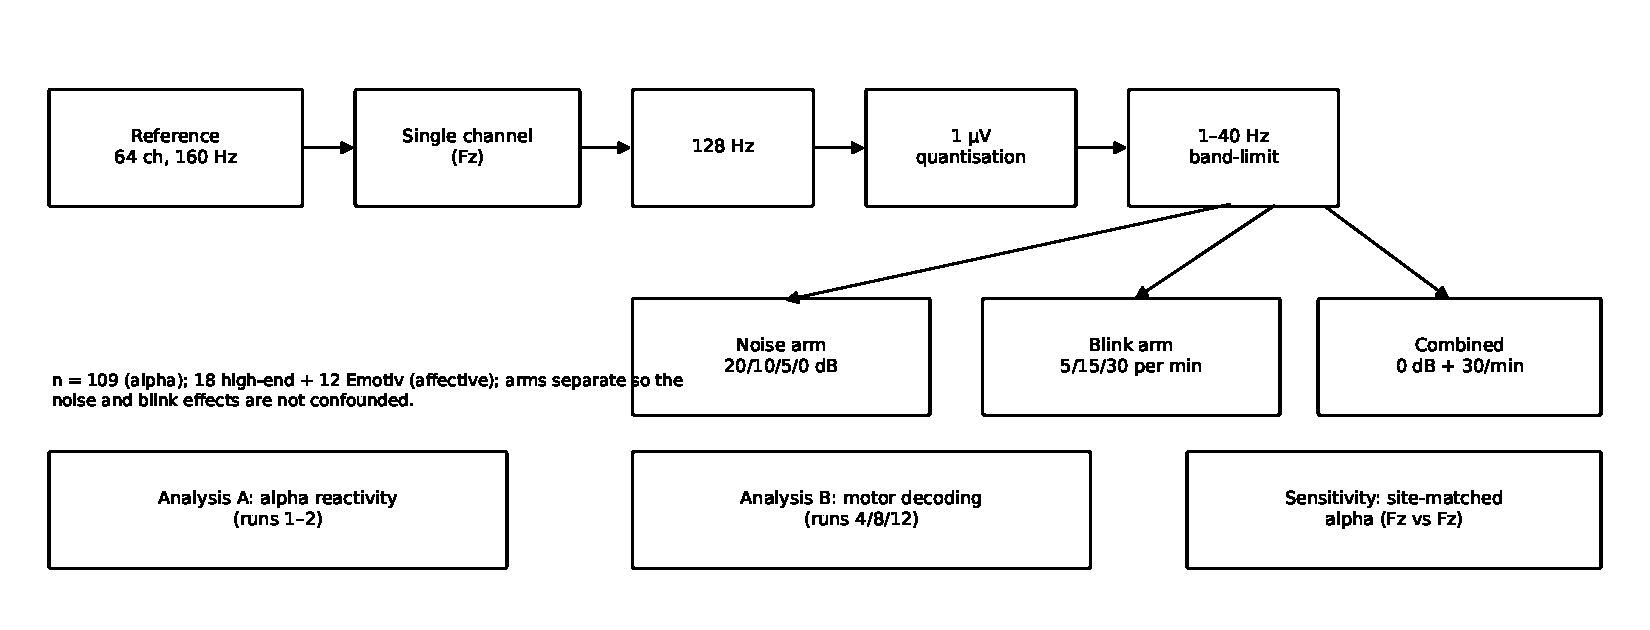
\includegraphics[width=\linewidth]{figures/fig1_pipeline.pdf}
  \caption{Degradation tree. The reference is the full-montage recording; the
  single-channel chain is cumulative, while the noise and blink arms branch from the
  fully degraded chain and are analysed separately.}
  \label{fig:pipeline}
\end{figure}

\subsection*{Noise is the constraint that matters; blinks alone do not shift alpha reactivity}
Noise produced a monotonic dose-response: $0.76$ at 20\,dB, $0.71$ at 10\,dB, $0.60$
at 5\,dB and $0.38$ at 0\,dB. Relative to the clean single-channel chain (the correct
baseline for an incremental contamination), the geometric retention was $0.99$, $0.94$,
$0.85$ and $0.68$; relative to the full-montage reference it was $0.86$, $0.82$, $0.73$
and $0.59$. The incremental paired contrasts
against the clean chain (which isolate the noise manipulation) were $-0.008$
($[-0.011, -0.006]$) at 20\,dB, $-0.064$ ($[-0.075, -0.052]$) at 10\,dB, $-0.169$
($[-0.197, -0.140]$) at 5\,dB and $-0.384$ ($[-0.441, -0.328]$) at 0\,dB; all survive
Benjamini--Hochberg correction across the condition family ($q<0.001$). The three blink arms were almost identical to
the clean chain ($0.77$ at 5 and 15/min, $0.77$ at 30/min). The incremental contrast (30 blinks/min minus
clean chain) was $-0.002$ ($[-0.003, -0.001]$; $q=0.0005$), a change of about 0.2\% that
is statistically detectable but negligible in size; the combined arm ($0.39$) was driven
by the 0\,dB noise it contains. The injected template has almost no energy in 8--12\,Hz
and the same rate was added to both conditions, so this null is close to guaranteed by
construction and should be read as a model check, not as evidence about real blinks;
ocular artifacts are known to bias broadband power in ways this additive model does not
represent \cite{hagemann2001ocular}.
The template has almost no 8--12\,Hz energy and the same rate is added to both
conditions, so the null is close to guaranteed and is not evidence about real ocular
contamination \cite{gratton1983ocular,croft2000ocular,whitham2007emg}.

\begin{figure}[H]
  \centering
  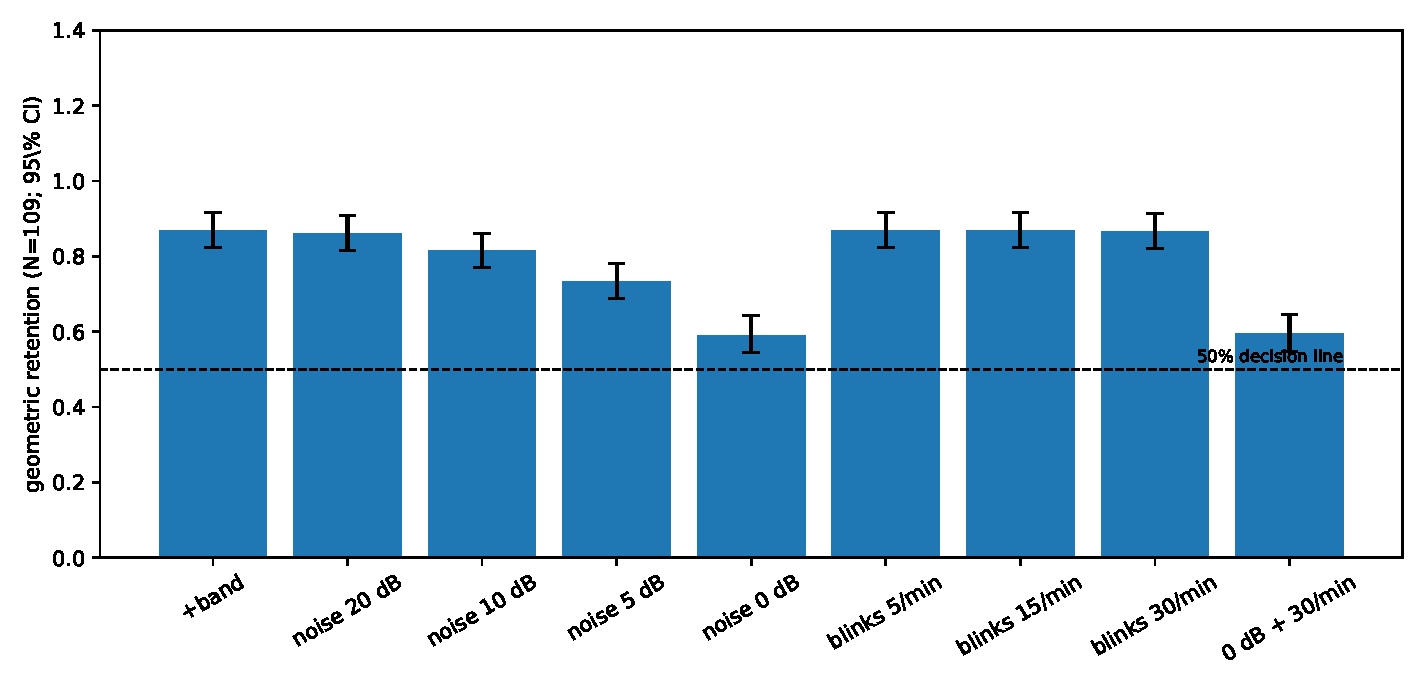
\includegraphics[width=0.85\linewidth]{figures/fig2_retention.pdf}
  \caption{Alpha reactivity retained relative to the clean single-channel chain, by
  condition ($N=109$; geometric retention and 95\% CI). The dashed line is the planned
  50\% decision threshold. Noise reduces retention monotonically; the blink arm is a
  model check and is not a real-blink test.}
  \label{fig:retention}
\end{figure}

\subsection*{Affective decoding survives a full montage but not one electrode}
Table~\ref{tab:affective} reports the affective arm on the high-end BrainVision
recordings (18 recordings from 20 participants; about 10 trials per quadrant). From the
full montage, valence was decoded at $0.69$ ($[0.62, 0.76]$), arousal at $0.68$
($[0.60, 0.75]$) and the four quadrants at $0.58$ ($[0.49, 0.67]$); the binary
intervals exclude chance and the four-class interval is above it. From the same data
reduced to the single-channel chain, valence showed no significant evidence of above-chance decoding ($0.52$; $[0.47, 0.57]$, $p=0.45$)
--- arousal to $0.56$ ($[0.50, 0.62]$), which remains above chance but far below the
montage, and the four quadrants to $0.34$ ($[0.27, 0.41]$). The paired full-minus-single
differences were $+0.17$ ($[0.10, 0.24]$) for valence, $+0.12$ ($[0.03, 0.20]$) for
arousal and $+0.24$ ($[0.14, 0.34]$) for the four quadrants, so the collapse is not
just a loss of significance.

A low-cost 14-channel Emotiv headset decoded the same targets at $0.67$
($[0.57, 0.77]$) for valence, $0.71$ ($[0.63, 0.79]$) for arousal and $0.56$
($[0.46, 0.67]$) for the four quadrants. On the 12 participants present in both
datasets, the low-cost minus high-end difference was $-0.07$ ($[-0.21, 0.08]$) for
valence, $+0.05$ ($[-0.05, 0.15]$) for arousal and $-0.04$ ($[-0.21, 0.12]$) for the
four quadrants. These differences are not statistically distinguishable from zero, but
a $\pm 10$-point equivalence test does not pass either (TOST $p=0.31$, $0.14$ and
$0.23$), so we describe the low-cost device as performing at a similar
level in this sample, not that equivalence has been established.

\begin{table}[H]
  \centering
  \caption{Affective decoding by acquisition representation: high-end full montage
  ($N=18$ recordings), low-cost 14-channel Emotiv ($N=12$), and high-end data
  reduced to one degraded channel ($N=18$). Balanced accuracy with 95\% CI;
  chance 0.50 (binary) and 0.25 (four-class).}
  \label{tab:affective}
  \begin{tabular}{lccc}
    \hline
    Target & High-end montage & Low-cost 14 ch & Single channel \\
    \hline
    Valence & 0.69 [0.62, 0.76] & 0.67 [0.57, 0.77] & 0.52 [0.47, 0.57] \\
    Arousal & 0.68 [0.60, 0.75] & 0.71 [0.63, 0.79] & 0.56 [0.50, 0.62] \\
    Four quadrants & 0.58 [0.49, 0.67] & 0.56 [0.46, 0.67] & 0.34 [0.27, 0.41] \\
    \hline
  \end{tabular}
\end{table}


\begin{figure}[H]
  \centering
  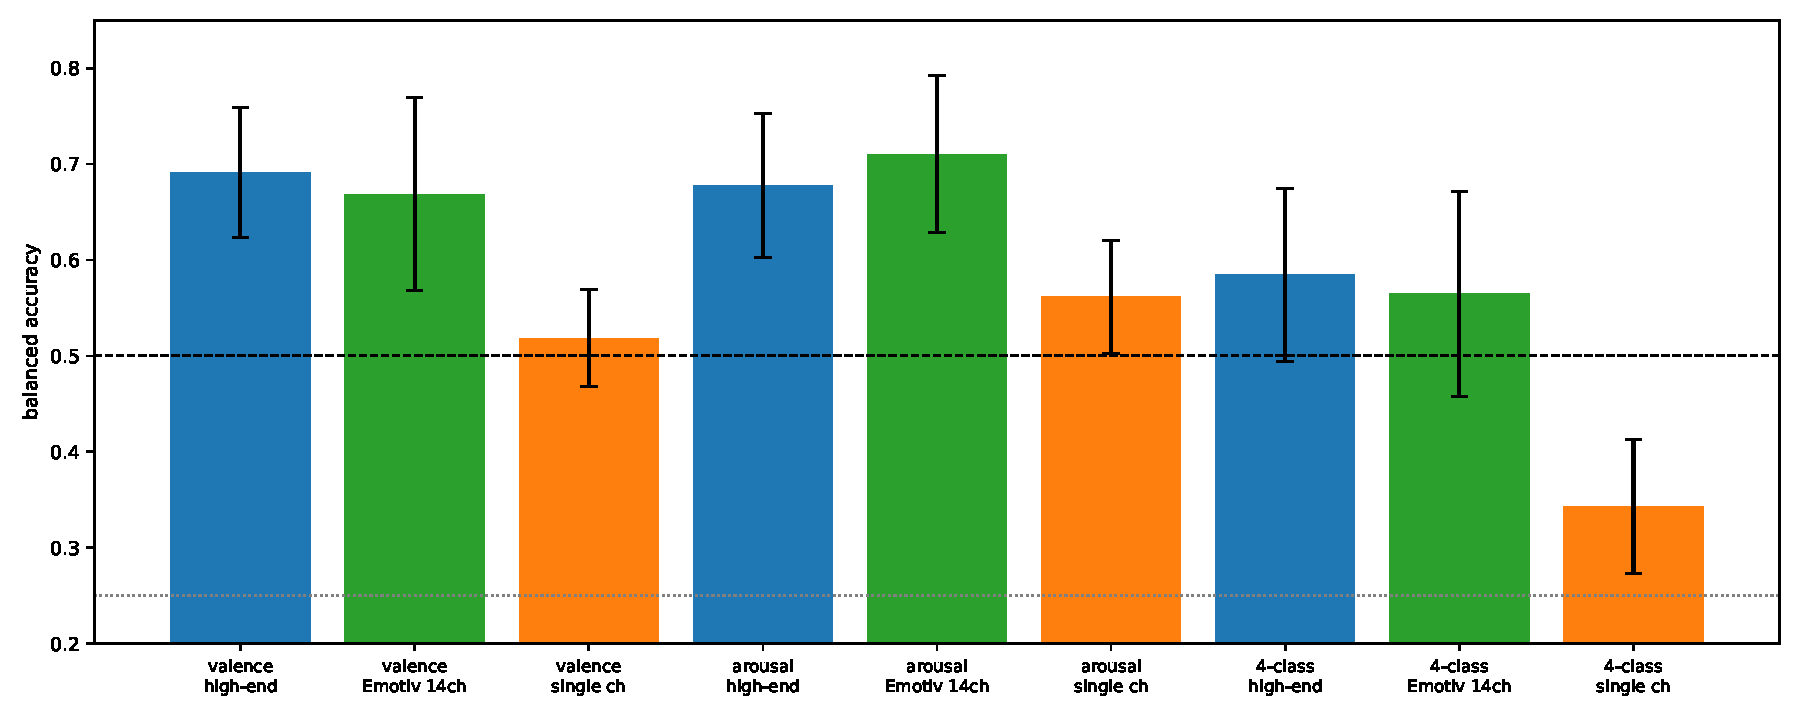
\includegraphics[width=0.9\linewidth]{figures/fig3_affective.pdf}
  \caption{Affective decoding by acquisition representation: high-end montage,
  low-cost 14-channel Emotiv and single-channel chain. Dashed and dotted lines mark
  chance for binary (0.50) and four-class (0.25) targets.}
  \label{fig:affective}
\end{figure}

\subsection*{Decomposing the affective collapse: representation, site and band}
The chain that is harmless for alpha is also harmless for affective decoding
(Table~\ref{tab:decomp}): resampling to 128\,Hz, quantisation and band-limiting left
four-class accuracy at $0.58$--$0.59$ and valence at $0.69$--$0.70$. The loss appears
when the representation becomes one electrode. Valence was not distinguishable from
chance at any of the four sites ($0.51$--$0.53$ at Fz, Cz, Pz and Oz); four-class
accuracy was $0.33$--$0.38$, above the $0.25$ chance level but far below the montage;
and arousal was weakly above chance at Fz, Pz and Oz before correction ($0.56$--$0.57$;
unadjusted $p\approx0.04$) but not at Cz ($0.56$, $[0.49, 0.62]$). The single-Fz arousal
value survives the six-contrast affective family ($q=0.0496$) but not the 12-test site
sweep ($q\approx0.079$); we therefore treat the site-level arousal pattern as
exploratory. With only four midline sites and three features per site, the
bounded claim is that none of these single-electrode representations approached the
montage, not that every possible electrode would fail.

A band control changes the interpretation of the full-montage result. With only theta
and alpha features the full montage decoded valence at $0.60$ ($[0.54, 0.66]$) and the
four quadrants at $0.46$ ($[0.38, 0.53]$), whereas beta-only features retained $0.70$
($[0.61, 0.79]$) and $0.62$ ($[0.53, 0.71]$). A substantial part of the
full-montage affective advantage therefore sits in the beta band, where EMG
contamination is a known concern \cite{whitham2007emg,goncharova2003emg}. Because
beta-only decoding was at least as high as the full montage ($0.70$ vs $0.69$ for
valence, $0.62$ vs $0.58$ for four-class), we do not interpret the montage advantage as
purely additive cortical information, and we did not measure EMG directly. This is an
interpretation, not a tested mechanism.

\begin{table}[H]
  \centering
  \caption{Decomposition of affective decoding (18 high-end recordings; balanced
  accuracy). Chance is 0.50 for valence/arousal and 0.25 for four-class.}
  \label{tab:decomp}
  \begin{tabular}{lccc}
    \hline
    Representation & Valence & Arousal & Four-class \\
    \hline
    Full montage, all bands & 0.69 & 0.68 & 0.58 \\
    Full montage, theta+alpha only & 0.60 & 0.63 & 0.46 \\
    Full montage, beta only & 0.70 & 0.70 & 0.62 \\
    128\,Hz / quantised / band-limited & 0.70 & 0.68 & 0.58 \\
    Single Fz & 0.52 & 0.56 & 0.34 \\
    Single Cz & 0.51 & 0.56 & 0.38 \\
    Single Pz & 0.52 & 0.56 & 0.33 \\
    Single Oz & 0.53 & 0.57 & 0.35 \\
    \hline
  \end{tabular}
\end{table}


\begin{figure}[H]
  \centering
  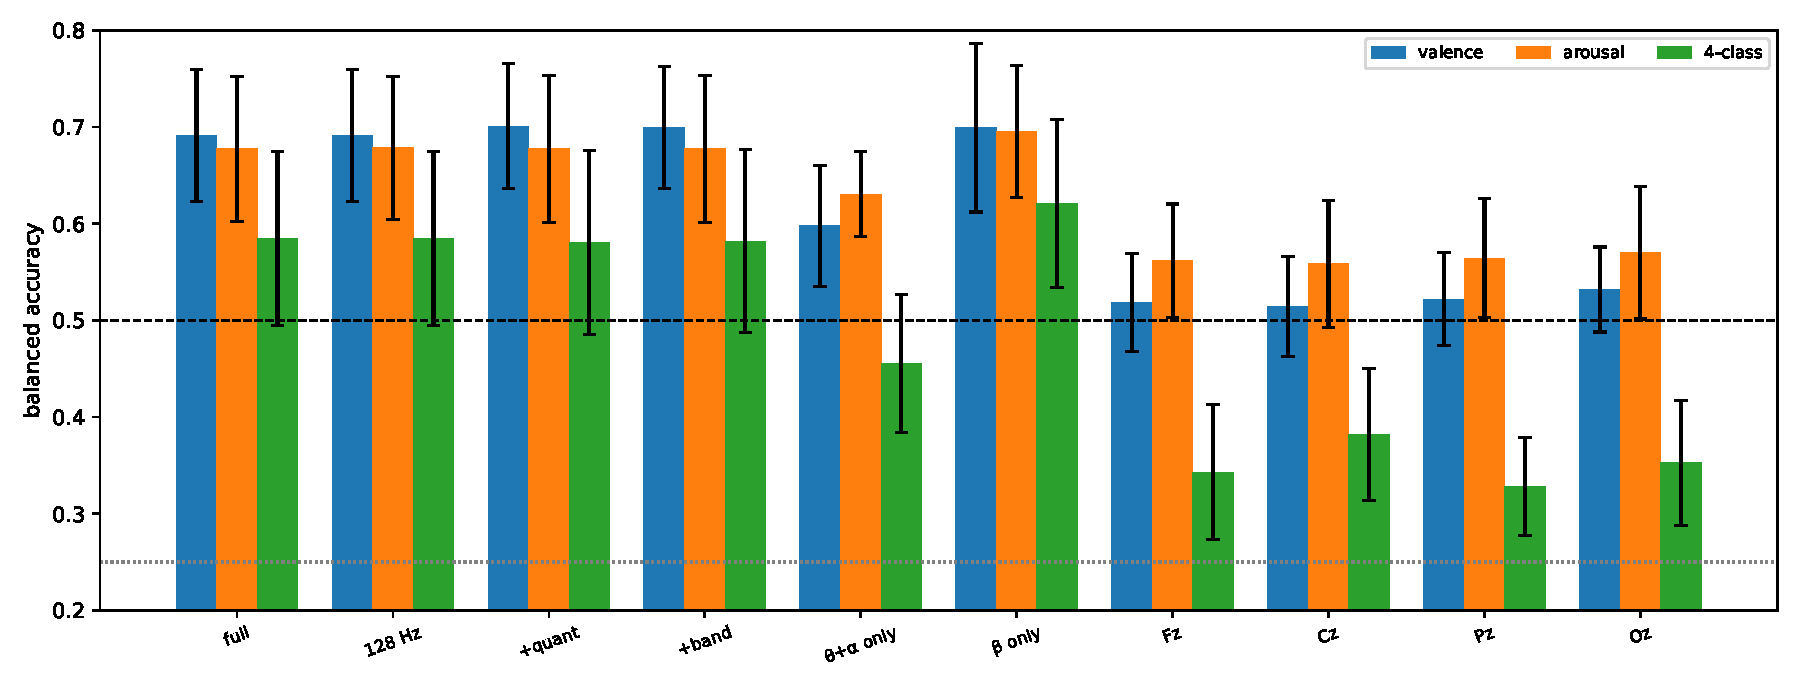
\includegraphics[width=\linewidth]{figures/fig4_decomp.pdf}
  \caption{Decomposition of affective decoding by acquisition step and band. The
  dashed and dotted lines mark chance for binary (0.50) and four-class (0.25) targets.}
  \label{fig:decomp}
\end{figure}

\subsection*{Reliability depends on the timescale}
Short-lag stability of consecutive 2\,s alpha windows was $r_{SB}=0.016$
($[-0.08, 0.11]$; $N=109$). This is a short-lag stability measure, not a classical
reliability coefficient: odd and even 2\,s windows are separated by about two
seconds. It says
that a momentary alpha estimate is noisy and is consistent with zero. In the ten-subject
subset with three repeated imagined-hand runs, block-level alpha power had
ICC(2,1)$=0.92$, which captures stable between-subject differences. The two are not
contradictory, and neither is a test--retest coefficient across sessions; published
single-channel test--retest work reports ICCs of roughly 0.76--0.85 for eyes-closed
relative power \cite{rogers2016reliability}, but on a different design.

\subsection*{Exploratory motor decoding was inconclusive}
In the ten-subject subset with imagery runs, balanced accuracy for imagined
left/right hand was $0.51$ ($[0.47, 0.56]$) at Fz and $0.54$ ($[0.46, 0.62]$) at the
full montage; a CSP reference reached $0.52$ ($[0.41, 0.63]$) and a sensorimotor subset
$0.55$ ($[0.44, 0.66]$). Every interval includes chance, and the full-montage decoder
has more features than trials (64 channels, 45 trials). Figure~\ref{fig:decoding} shows the distribution of these accuracies.
Because the reference decoder itself did not exceed chance, this arm cannot test the
decoding hypothesis; it is reported as \textbf{invalid}, not merely inconclusive, and
is not used for any claim.

\begin{figure}[H]
  \centering
  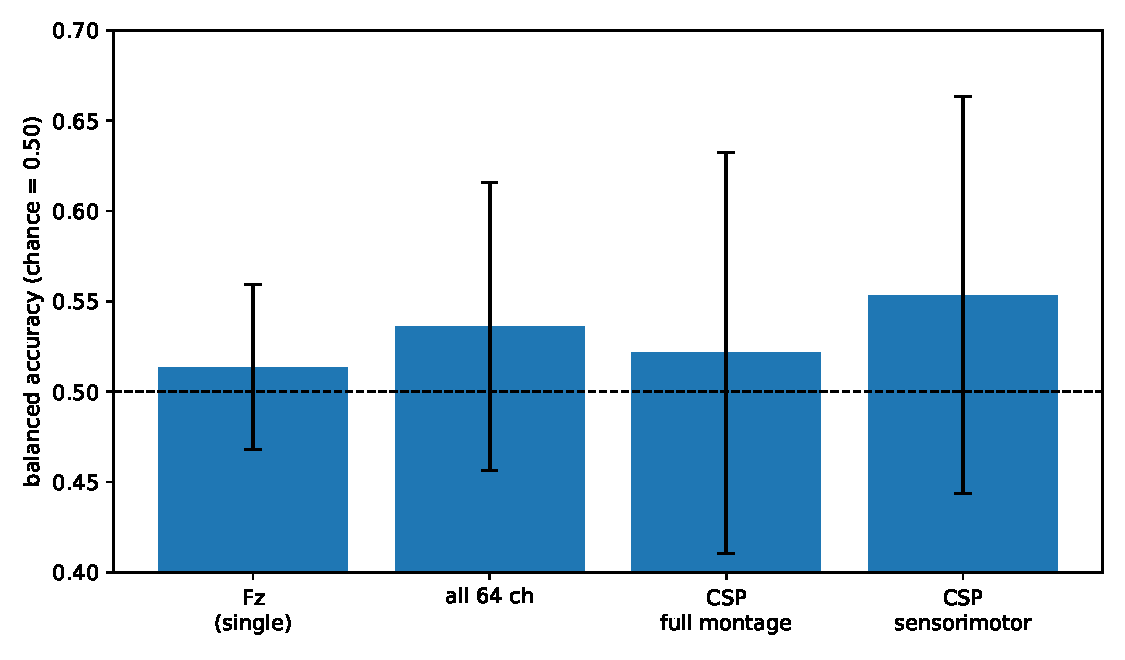
\includegraphics[width=0.9\linewidth]{figures/fig5_decoding.pdf}
  \caption{Exploratory motor-imagery decoding ($N=10$), balanced accuracy by
  representation. All intervals include chance (0.50).}
  \label{fig:decoding}
\end{figure}

\subsection*{Decision matrix}
Table~\ref{tab:decision} applies the planned 50\% retention rule to the outcomes
that were estimated.

\begin{table}[H]
  \centering
  \caption{Claim-level verdicts.}
  \label{tab:decision}
  \begin{tabular}{p{0.40\linewidth}p{0.28\linewidth}p{0.24\linewidth}}
    \hline
    Claim & Evidence & Verdict \\
    \hline
    Alpha reactivity survives the acquisition chain & Same-site reactivity retention lower bound 0.9996 & Supported \\
    Alpha reactivity survives 20--5\,dB noise & Clean-chain retention lower bounds 0.99, 0.93, 0.82 & Supported \\
    Alpha reactivity survives 0\,dB noise & Clean-chain retention 0.68 [0.64, 0.72] & Supported (attenuated) \\
    Combined 0\,dB + 30 blinks/min & Clean-chain retention 0.68 [0.65, 0.71] & Supported (attenuated) \\
    Blinks bias alpha reactivity & Clean-chain retention 0.998 in a spectrally orthogonal, symmetric model & Not a real-blink test (H1 untested) \\
    Pre-specified 60\% balanced-accuracy floor & Valence full passes (lower 0.62); four-class full fails (lower 0.49); Emotiv valence fails (lower 0.57); arousal full/Emotiv pass & Mixed; reported as auxiliary criterion \\
    Single-trial motor decoding above chance & Reference decoder did not exceed 0.50 & Invalid (not testable) \\
    Momentary individual-level alpha reliability & Short-lag stability $r_{SB}=0.016$ & Not supported \\
    Stable individual alpha level & ICC across runs 0.92 (no CI) & Supported (block-level) \\
    \hline
  \end{tabular}
\end{table}

\noindent
\textbf{Status.} The alpha arm uses the full 109-subject dataset. The
affective arm uses 18 high-end recordings and 12 low-cost Emotiv recordings; the Emotiv
alignment relies on wall-clock timestamps and 8 participants are dropped. The
full-montage affective advantage is partly beta-band and may include a muscular
contribution. The motor arm is invalid (reference at chance) and underpowered; H5 is untested. These scope limits are
stated in the Discussion and are not treated as results.


\section{Discussion}
% 05-discussion — v4.0
\subsection*{What survived, and what did not}
The two halves of the benchmark give different answers. Alpha reactivity survives the
acquisition chain almost intact: at the same electrode, the chain costs 0.01\% of the
effect. What costs alpha is the choice of electrode. Fz has about 58\% of the
eyes-closed alpha power of a posterior average, and this difference is a property of the
scalp, not of the electronics. Noise also matters, and it matters in a predictable way:
the effect declines steadily and reaches 59\% of the reference at 0\,dB. Bandwidth,
sampling rate and quantisation, the specifications usually printed on a consumer
headset's box, changed the 8--12\,Hz estimate by a negligible amount.

Affective decoding behaves differently. With the full montage, valence, arousal and
four-quadrant classification are above chance. With one electrode they are not: valence
is undetectable, arousal is weak, and four-class accuracy falls to 0.34. The contrast is
not a statement about broad alpha versus distributed affect. The two analyses use
different effect sizes, different numbers of trials and different estimators, and the
alpha ratio is partly invariant to the operations we applied. The useful conclusion is
narrower: within this benchmark, the acquisition chain does not limit alpha, but it does
limit affective decoding once the spatial representation is reduced to one site.

\subsection*{Where the affective result goes}
The decomposition helps. Resampling, quantisation and band-limiting leave full-montage
accuracy unchanged. The loss appears when the data become one electrode, and it appears
at all four midline sites we tried. Valence is not distinguishable from chance at Fz,
Cz, Pz or Oz, and four-class accuracy stays between 0.33 and 0.38. Arousal is the
exception: it remains weakly above chance at Fz, Pz and Oz before correction, though not
after correction across the site sweep. We treat the site sweep as exploratory.

The band control changes how the montage result should be read. With only theta and alpha
features, valence falls to 0.60 and four-class accuracy to 0.46. Beta-only features give
0.70 and 0.62, and beta-only is at least as good as the full montage. Beta is also where
EMG contamination is most likely \cite{whitham2007emg,goncharova2003emg}. We did not
record EMG or test a paired beta-versus-theta/alpha difference, so the result is an
interpretation: part of the montage advantage may be muscular rather than cortical. That
possibility should be ruled out before the montage number is used as a neural benchmark.

The low-cost Emotiv arm is a useful sanity check. Its accuracy is close to the high-end
montage on the 12 participants present in both datasets, and the matched differences are
small. The equivalence test does not pass, however, so the appropriate description is
"similar in this sample", not "equivalent". The comparison also mixes channel count,
feature count, recording units, epoch window and condition arm, and eight participants
are missing from the Emotiv analysis. It is a check, not a device validation.

\subsection*{What this means for reporting}
The first lesson is about reference choice. Comparing one electrode with a whole-head
average confounds channel count with electrode site, and a benchmark that does so will
understate what a single channel retains. The correction is simple: compare the same
site before and after degradation. Reference and site dependence of scalp power is not a
new observation \cite{hagemann2001reference}; what is new here is the size of the effect
for a single-channel benchmark, and the recommendation to make same-site comparison the
default.

The second lesson is about the site itself. Fz is a convenient research midline
electrode, but most single-electrode consumer devices record at the forehead: Fp1 in
NeuroSky/MindWave and AF7/AF8 in Muse \cite{krigolson2017muse,cannard2021muse}. Frontal
sites have less posterior alpha and more ocular and muscle contamination, so the 42\%
site cost we measured is probably an underestimate for those devices. The consumer-EEG
reliability comparison we cite is also at Fp1 \cite{rogers2016reliability}, not Fz. The
single-channel affective failure is established here for Fz, Cz, Pz and Oz, not for every
possible electrode.

The third lesson is about timescale. A 2\,s alpha window is a noisy estimate of a
momentary state; the odd--even correlation is a short-lag stability measure, not a
reliability coefficient, and its value near zero should not be read as "alpha is
unreliable". Block-level alpha power was much more stable (ICC 0.92). A product that
reports "your alpha right now" and a study that reports a stable individual difference
are making different claims.

\subsection*{Limitations}
The alpha arm uses all 109 subjects, but only the first 30 have the repeated motor runs
needed for the ICC estimate; the ICC therefore rests on a small subset and has no
confidence interval. The affective arm uses 18 high-end recordings, and the Emotiv arm
covers 12 participants. The Emotiv signal is in device units, its epoch window differs
slightly from the BrainVision epochs, and the archive's two condition arms are not
distinguished. We did not measure a real single-channel device, so the single-channel
condition is a simulation of that device, not the device itself. The blink model is
additive, spectrally orthogonal to alpha, and applied equally to both conditions; it
cannot test the real ocular interaction, and the pre-specified blink hypothesis is
therefore untested. Artifact handling is minimal: no ICA or Autoreject, so the beta-band
features may be contaminated. The affective labels are normative IAPS categories rather
than participants' own ratings, and we did not test picture-level generalisation or a
label-permutation null. Only four midline sites were swept, and the single-channel
condition has three features against 198 for the full montage, so the representation
comparison confounds information with dimensionality. The 0\,dB level is defined on
broadband variance, the in-band signal-to-noise ratio is not reported, and the ratio
estimator can compress the effect. Eight of 109 subjects had a negative reference
reactivity, which is expected for a resting-state contrast but limits the precision of
the mean. The analysis plan was not registered; several pre-specified items (Fp1/Cz
sensitivity, the 60\% floor, AUC and median-split outcomes) were changed or dropped, and
the study is exploratory in the strict sense. The motor arm is invalid, not merely
underpowered, because its reference decoder did not exceed chance. Finally, the
equivalence test uses a small sample and a margin that is wide relative to the observed
differences.

\subsection*{Where to go next}
The obvious next step is a real single-channel device. A small study with a consumer
headset, raw samples and the same pipeline would show whether the simulation is
realistic, and whether the site cost is larger at the forehead, as we expect. A second
step is to measure EMG or add a high-frequency control to separate muscular from
cortical contributions to the beta-band result. A third is to register the analysis
plan and repeat the alpha arm with a pre-specified decision rule. None of these requires
new theory; they require better measurement, which is the point of the benchmark.


\section{Conclusion}
% 06-conclusion — v2.0
We presented a reproducible degradation benchmark for single-channel and low-cost EEG
and applied it to two open datasets. The results are conditional and, we think, useful.
Alpha reactivity survived the acquisition chain almost intact once the reference was
taken at the same electrode (99.99\% retained; a ratio-of-ratios outcome, so gain-like
steps cancel by construction), whereas the electrode-site decision cost
about 42\% of eyes-closed alpha power and sensor noise reduced the effect monotonically,
to about 0.59 of the reference at 0\,dB. Affective valence was decodable from a full high-end
montage ($0.69$) but was not detected from a single electrode ($0.52$); arousal survived
weakly ($0.56$ above chance but far below $0.68$), and four-class accuracy fell to $0.34$ (above chance but far below the montage). A
low-cost 14-channel headset performed at a similar level to the high-end montage without
passing a formal equivalence test. Decomposition showed that the acquisition chain was
harmless, that valence was not distinguishable from chance at any single site and the
four-class result stayed far below the montage, and that beta-band
features carried part of the full-montage advantage --- a result that cautions against
reading the montage number as purely cortical.

The deliverable is a decision matrix, a single-channel reporting checklist, and an open,
seeded analysis pipeline that turns public data into the reported numbers. The next
version requires the full subject sample, a real single-channel device, a validated
artifact model, registration of the analysis plan, and a larger equivalence study. The
value of the exercise is that it replaces a plausible story ("single channels lose
information") with a measured one: what a single electrode can and cannot show depends
on the analysis, the site and the band, and that boundary can be mapped.


\section*{Use of generative AI}
Generative AI was used as an analysis and writing tool. The assistant (DeepSeek Harness,
DeepSeek model) wrote and debugged analysis code, ran the statistical pipeline, generated
figures and tables from the archived data, checked citation metadata against Crossref and
DataCite, simulated reviewer feedback during revision, and edited the prose. Every number
reported here was computed by the scripts in the repository and checked against the
archived JSON; every cited reference was checked against a DOI record. The AI did not
generate or alter data, did not produce any image presented as experimental data, and is
not an author. The author takes full responsibility for the content and conclusions.

\section*{Data and code availability}
All datasets are public. The EEG Motor Movement/Imagery Dataset is available from
PhysioNet (\href{https://doi.org/10.13026/C28G6P}{doi:10.13026/C28G6P}). The affective
dataset is available from Zenodo under CC BY 4.0
(\href{https://doi.org/10.5281/zenodo.14787743}{doi:10.5281/zenodo.14787743}). DEAP was
not used: its download page was unreachable during this work, and the DREAMER record is
access-restricted \cite{katsigiannis2018dreamer}. The analysis repository (degradation pipeline, analysis scripts,
seeds, environment file and the JSON files behind every number) is public at
\href{https://github.com/curiousbrutus/EEG-Benchmark}{github.com/curiousbrutus/EEG-Benchmark}
and mirrored on the OSF project page \href{https://osf.io/8wxqj/}{osf.io/8wxqj}. The
archived version is deposited at Zenodo under DOI
\href{https://doi.org/10.5281/zenodo.23976432}{10.5281/zenodo.23976432}. The commit hash
used for this draft is recorded in \texttt{results/data\_manifest.json}. The single-channel
reporting checklist is included as \texttt{CHECKLIST.md}. No new human participants were
recorded.

\section*{Author contributions}
Conceptualization, methodology, software, analysis, writing: E.G.

\section*{Acknowledgements}
No funding was received for this work. The author declares no competing interests.

\bibliographystyle{plain}
\bibliography{refs}

\end{document}
